\documentclass[a4paper]{article}
%%%%%%%%%%%%%%%%%%%%%%%%%%%%%%%%%%
\usepackage{tabularx}
\usepackage{float}

% \usepackage[demo]{graphicx}
\usepackage{subfig}

\usepackage{fancyhdr}
% Package for making LaTeX properly handle utf8 characters set and danish language rules
\usepackage[utf8]{inputenc}
\usepackage[danish]{babel}
%%%%%%%%%%%%%%%%%%%%%%%%%%%%%%%%%%
% Package for changing to a nicer font 
\usepackage [T1]{fontenc}
%%%%%%%%%%%%%%%%%%%%%%%%%%%%%%%%%%
% Package for conctroling the text area
\usepackage[margin=2.5cm]{geometry}
%%%%%%%%%%%%%%%%%%%%%%%%%%%%%%%%%%
% Package for importing PDF
\usepackage{pdfpages}
%%%%%%%%%%%%%%%%%%%%%%%%%%%%%%%%%%
% Math fonts:
\usepackage{amsfonts} 
%%%%%%%%%%%%%%%%%%%%%%%%%%%%%%%%%%
% Package for inserting clickable hyperlinks in pdf versions as produced by pdflatex
\usepackage{hyperref}
%%%%%%%%%%%%%%%%%%%%%%%%%%%%%%%%%%
% Package for including figures. TeX and thus LaTeX was developped before the existence of directory file-structures, but the graphicspath let's you add directories, that the \includegraphics will search.
\usepackage{graphicx}
\graphicspath{{figures/}{anotherFigureDirectory/}}
%%%%%%%%%%%%%%%%%%%%%%%%%%%%%%%%%%
% Package for typesetting programs. Listings does not support fsharp, but a little modification goes a long way
\usepackage{listings}
\usepackage{color}
\usepackage[shortlabels]{enumitem}
\definecolor{bluekeywords}{rgb}{0.13,0.13,1}
\definecolor{greencomments}{rgb}{0,0.5,0}
\definecolor{turqusnumbers}{rgb}{0.17,0.57,0.69}
\definecolor{redstrings}{rgb}{0.5,0,0}
\lstdefinelanguage{FSharp}
                {morekeywords={let, new, match, with, rec, open, module, namespace,type, of, member, and, for, in, do, begin, end, fun, function, try, mutable, if, 
then, else},
    keywordstyle=\color{bluekeywords},
    sensitive=false,
    morecomment=[l][\color{greencomments}]{///},
    morecomment=[l][\color{greencomments}]{//},
    morecomment=[s][\color{greencomments}]{{(*}{*)}},
    morestring=[b]",
    stringstyle=\color{redstrings}
    }
%%%%%%%%%%%%%%%%%%%%%%%%%%%%%%%%%%
% Package for extended math settings, e.g. \eqref
\usepackage{amsmath}
\pagestyle{fancy}
\usepackage[utf8]{inputenc}

\title{Mærsk emission}
\author{Alexander Husted}
\date{February 2023}
\fancyhead[L]{Mærsk emission}
\begin{document}
\maketitle

\large % Makes text larger
\vspace{3cm} % space

\begin{center} 
{\setlength\arrayrulewidth{2pt}
\begin{tabular}{r|p{9.8cm}}
\colorbox{cyan}{\textcolor{white}{\bf Page 2}}      
& \textbf{\underline{Introduction}} \: The document's overall structure will be defined, and the point of departure will be explained.         \\[2cm]

%\colorbox{udc}{\textcolor{white}{\bf GRADO}} & Dual en Ingeniería Eléctrica    \\[1cm]
\colorbox{cyan}{\textcolor{white}{\bf Page 3}}       
    & \textbf{\underline{SQL}} Basic SQL queries to extract different tables of data.   \\[1cm]
\colorbox{cyan}{\textcolor{white}{\bf Page 6}}  
    & \textbf{\underline{R}} Visualise and calculate data using data from the database.     \\[2cm]
\colorbox{cyan}{\textcolor{white}{\bf Page 7}}  
    &	\underline{\textbf{Appendix}} Contains code snippets from solutions..  \\[2cm]

\end{tabular}}
\end{center}
\normalsize
\newpage
\section{Introduction}
\begin{flushleft}
    The document will take point in a demo SQL database I created.   The main focus of the database \\
    (fig. ~\ref{fig:dataBase}) will be on the vessels and their environmental impact. Throughout the document, I will answer specific problems using a combination of SQL and R to create an impression of my current capabilities in the different fields. \newline \newline Mostly you'll be able to find the code under the problem as an answer, but longer code is stored as an appendix. The createDatabase script is the longest and can be found on https://github.com/Husted42/code/blob/main/projects/containerTransport/SQLscrips/createDB.sql \\
    Everything is thoroughly tested and runs as expected.
\end{flushleft}
 
\begin{figure} [h]
    \centering
    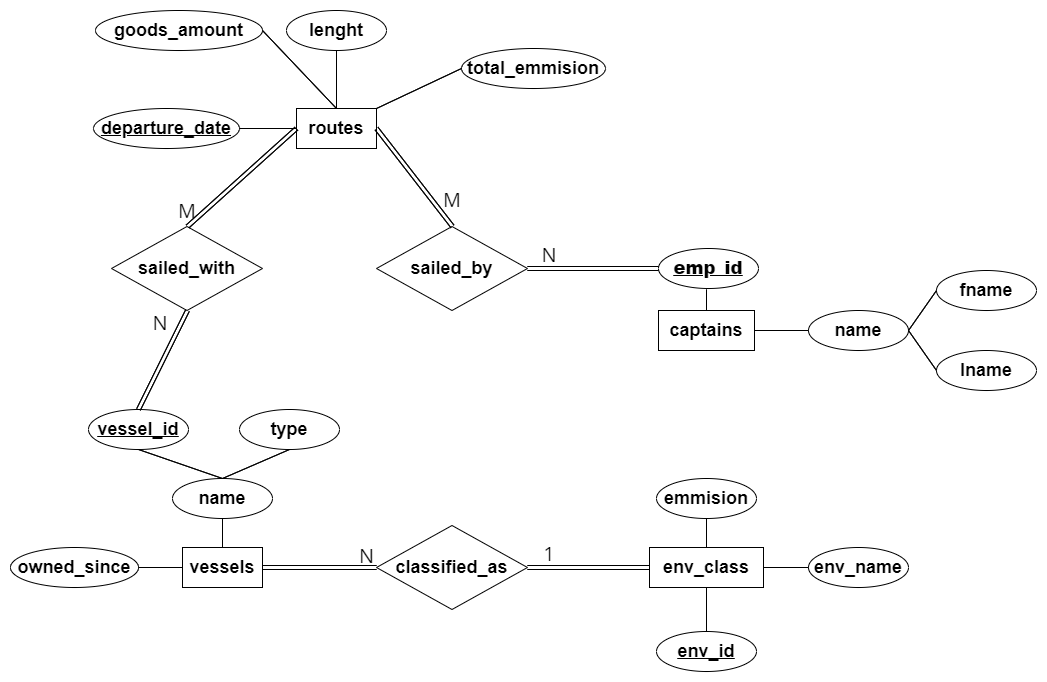
\includegraphics[width=1\linewidth]{assets/DB.png}
    \caption{DEMO database}
    \label{fig:dataBase}
\end{figure}

\newpage
\section{SQL}
This chapter will resolve problems using simple SQL queries and show a table as an output. The five main focus points are functions, nestedQueries, unions, wildcards, and joins.
\begin{flushleft}
    \textbf{Find the average total emission from each environmental class.}
    \begin{table}[!ht]
    \flushleft
    \begin{tabular}{|l|l|}
    \hline
        env\_name & averageEmmission \\ \hline
        A & 34330.0833 \\ \hline
        B & 49518.6000 \\ \hline
        C & 59295.0000 \\ \hline
        D & 74855.0000 \\ \hline
    \end{tabular}
    \end{table}
    \begin{figure} [h]
        \flushleft
        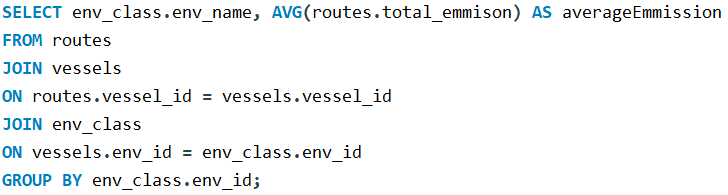
\includegraphics[width=0.8\linewidth]{code/SQLtotalEmmision.PNG}
        \label{fig:SQLtotalEmmision}
    \end{figure} \newline
    As expected, the better the environmental class, the lesser the average total emission.
\end{flushleft}

\begin{flushleft}
    \textbf{Find all the captains that have sailed longer than 9000 km. in a single route.}
    \begin{table}[!ht]
    \flushleft
    \begin{tabular}{|l|l|}
    \hline
        fname & lname \\ \hline
        Archibald & Haddock \\ \hline
        James & Hook \\ \hline
        Bartholomew & Roberts \\ \hline
    \end{tabular}
    \end{table}
    \begin{figure} [H]
        \flushleft
        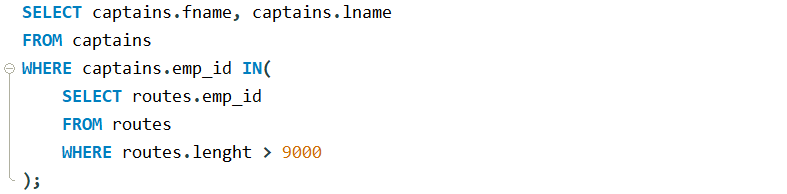
\includegraphics[width=1\linewidth]{code/SQLcaptainsLenght.PNG}
        \label{fig:SQLcaptainsLenght}
    \end{figure}
    Out of a total of 5 captains, 3 have experience with sailing routes longer than 9.000 kilometers.
\end{flushleft}
\newpage
\begin{flushleft}
    \textbf{Find all of the captains and vessels names.}
    \begin{table}[!ht]
    \flushleft
    \begin{tabular}{|l|l|}
    \hline
        fname & lname \\ \hline
        Archibald & Haddock \\ \hline
        James & Hook \\ \hline
        Ferdinand & Magellan \\ \hline
        Bartholomew & Roberts \\ \hline
        Ferdinand  & Nelson \\ \hline
        1 & KFM Gold \\ \hline
        2 & KFM Silver \\ \hline
        3 & Zode Silver \\ \hline
        4 & MST Gold \\ \hline
        5 & MST Bronze \\ \hline
        6 & LDS Gold \\ \hline
        7 & KFM Silver \\ \hline
        8 & Zode Gold \\ \hline
        9 & KFM Silver \\ \hline
        10 & MST Bronze \\ \hline
    \end{tabular}
    \end{table}
    \begin{figure} [H]
        \flushleft
        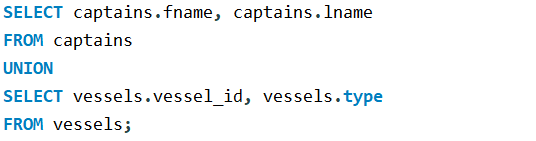
\includegraphics[width=0.7\linewidth]{code/SQLunion.PNG}
        \label{fig:SQLunion}
    \end{figure}
    For both the vessels and the captains, their names contain two different attributes. For the captains, it's fname and lname, and for vessels, it's vessel\_id and type.
\end{flushleft}

\begin{flushleft}
    {\bf Find all vessels bought in June and July.}
    \begin{table}[!ht]
    \flushleft
    \begin{tabular}{|l|l|l|l|}
    \hline
        vessel\_id & type & owned\_since & env\_id \\ \hline
        3 & Zode Silver & 1994-06-28 & 1 \\ \hline
        4 & MST Gold & 1995-07-30 & 1 \\ \hline
        9 & KFM Silver & 2003-07-03 & 1 \\ \hline
        10 & MST Bronze & 2008-06-09 & 4 \\ \hline
    \end{tabular}
    \end{table}
    \begin{figure} [H]
        \flushleft
        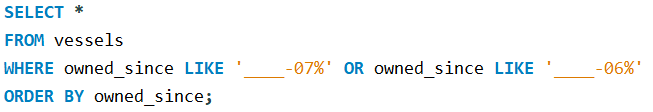
\includegraphics[width=0.8\linewidth]{code/SQLownedSince.PNG}
        \label{fig:SQLownedSince}
    \end{figure}
    The fictional vessels must go through service every year; the above four ships need to be serviced in either June or July.
\end{flushleft}
\newpage
\begin{flushleft}
{\bf Find the estimated emission from each vessel.} 
\begin{table}[!ht]
    \flushleft
    \begin{tabular}{|l|l|l|l|}
    \hline
        vessel\_id & type & env\_name & emmision \\ \hline
        1 & KFM Gold & A & 3.0 \\ \hline
        3 & Zode Silver & A & 3.0 \\ \hline
        4 & MST Gold & A & 3.0 \\ \hline
        6 & LDS Gold & A & 3.0 \\ \hline
        9 & KFM Silver & A & 3.0 \\ \hline
        2 & KFM Silver & B & 4.5 \\ \hline
        5 & MST Bronze & B & 4.5 \\ \hline
        7 & KFM Silver & C & 6.0 \\ \hline
        8 & Zode Gold & C & 6.0 \\ \hline
        10 & MST Bronze & D & 7.5 \\ \hline
    \end{tabular}
    \end{table}
    \begin{figure} [H]
        \flushleft
        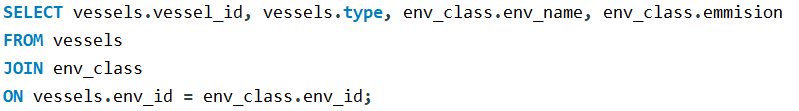
\includegraphics[width=1\linewidth]{code/SQLestimatedEmmision.PNG}
        \label{fig:SQLestimatedEmmision}
    \end{figure}
    When choosing which vessels to send out on the long routes, it's essential to know which vessels emit the least per kilometer.
\end{flushleft}
\newpage
\section{R}
\begin{flushleft}
    {\bf The stakeholders want to know the distribution of the environmental classes. Using R create two piecharts visualizing this distribution.} \\ Code can found in (appx. ~\ref{appendix:pieChart})
    \begin{figure} [H]%
        \centering
        {{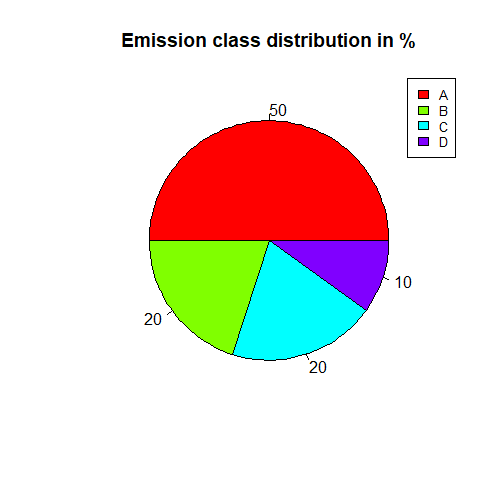
\includegraphics[width=0.4\linewidth]{assets/pieChart1.png} }}%
        \qquad
        {{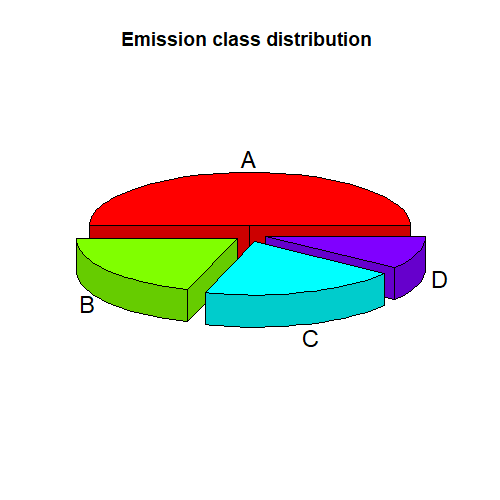
\includegraphics[width=0.4\linewidth]{assets/pieChart2.png} }}%
        \caption{pieCharts}%
        \label{fig:pieChart}%
    \end{figure}
\end{flushleft}

\begin{flushleft}
    {\bf There has been a problem with the latest trip. The sensor to measure emissions has broken down on the last shipment. Calculate the total emission.} \\
    The most obvious solution would be to multiply the length of the trip by the corresponding emission estimate per kilometer. But as seen in (fig. ~\ref{fig:EmmisionR})(appx. ~\ref{appendix:emmisionRcode}), the actual emission deviates from the estimated emission, and this is due to the amount of goods a vessel carries.
    \begin{figure} [H]%
        \centering
        {{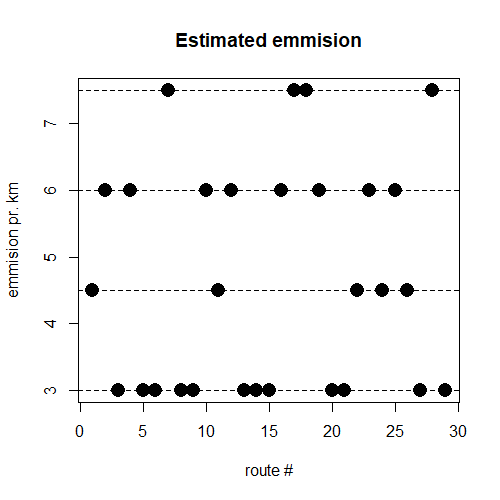
\includegraphics[width=0.4\linewidth]{assets/estimatedEmmision.png} }}%
        \qquad
        {{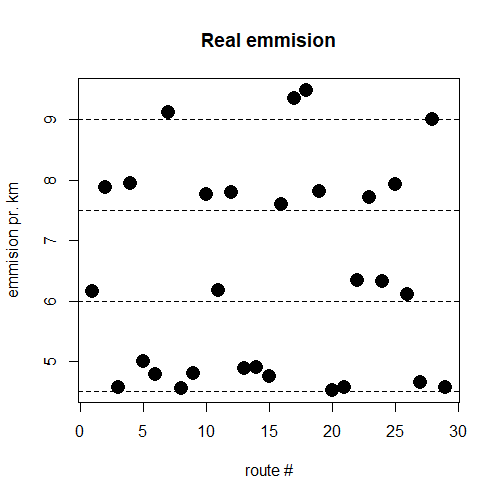
\includegraphics[width=0.4\linewidth]{assets/realEmmision.png} }}%
        \caption{emissionPlot}%
        \label{fig:EmmisionR}%
    \end{figure}

    A linear regression model can predict the outcome of real emission per kilometer if given data about previous routes. Therefore let $ X^{1}_{i} $ be amount of goods in tons, $ X^{2}_{i} $ be estimated emission in grams per kilometer and $ Y_i $ be real emission in gramsv per kilometer. The data $ (X^{1}_{1}, X^{2}_{1}, Y_1), ... , (X^{1}_{n}, X^{2}_{n}, Y_n) $ and: \\ $ X^{1}_{new} = 164 $ , $ X^{2}_{new} = 3 $ gets loaded into R. \newline \newline
    Using R, the predicted emission per kilometer is approximately 4.68 gram per kilometer. (appx. ~\ref{appendix:emmisionRcode2}) \\
    The last route had a length of 6582 kilometers. \\
    The latest route polluted $ 6582 \cdot Y_{new} = 30776.2 $ grams in total.
\end{flushleft}

\newpage
\section{Appendix}
\subsection{Code: Piecharts}
\label{appendix:pieChart}
SQL: 
\begin{figure} [H]
    \flushleft
    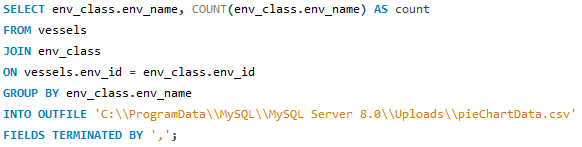
\includegraphics[width=1\linewidth]{code/pieSQL.PNG}
    \label{fig:Piechartss}
\end{figure} 
{\flushleft R:}
\begin{figure} [H]
    \flushleft
    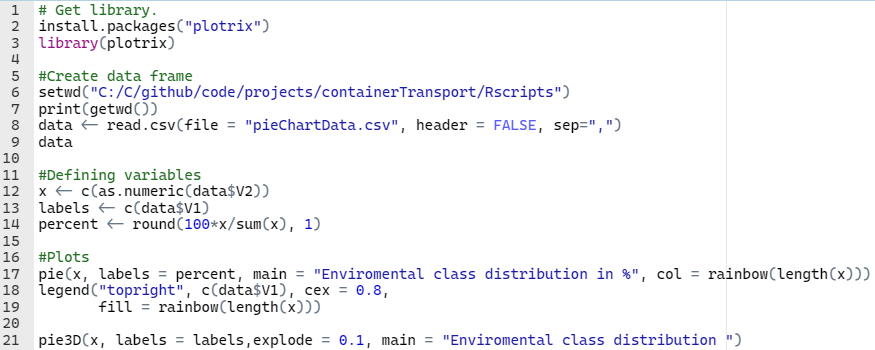
\includegraphics[width=1\linewidth]{code/pieR.PNG}
    \label{fig:piechart}
\end{figure}

\subsection{Code: Rplot emission}
\label{appendix:emmisionRcode}
\begin{figure} [H]
    \flushleft
    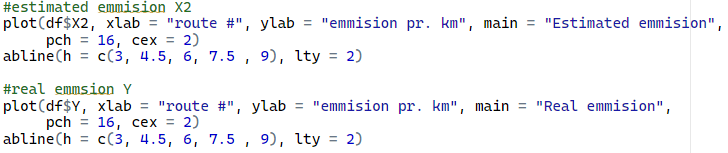
\includegraphics[width=1\linewidth]{code/RemmisionPlot.PNG}
    \label{fig:RemmisionPlot}
\end{figure}

\newpage
\subsection{Code: Emission prediction}
\label{appendix:emmisionRcode2}
SQL: 
\begin{figure} [H]
    \flushleft
    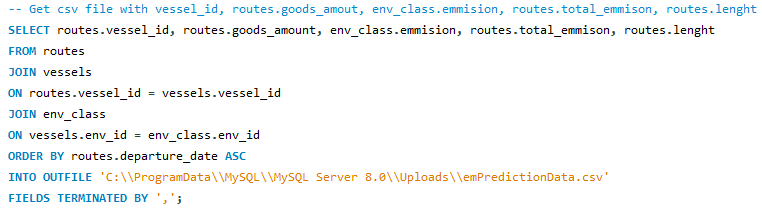
\includegraphics[width=1\linewidth]{code/SQLtoR.PNG}
    \label{fig:SQLtoR}
\end{figure} 
{\flushleft R:}
\begin{figure} [H]
    \flushleft
    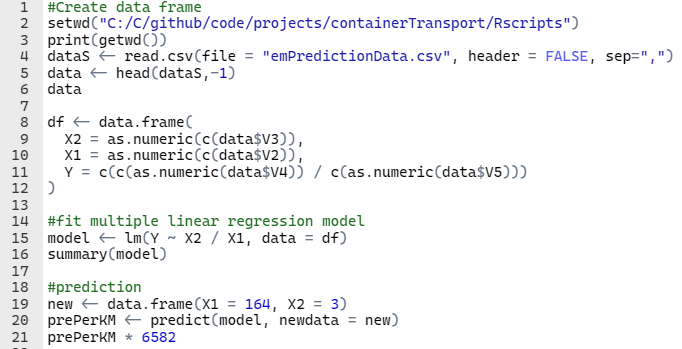
\includegraphics[width=1\linewidth]{code/Rpredict.PNG}
    \label{fig:Rpredict}
\end{figure}

\end{document}